% BSP Registry Tools — Technical Reference
% A4 LaTeX document
% Compile with: pdflatex bsp_registry_tools.tex
\documentclass[a4paper,11pt]{article}

% ── Encoding & fonts ──────────────────────────────────────────────────────────
\usepackage[T1]{fontenc}
\usepackage[utf8]{inputenc}
\usepackage{lmodern}

% ── Page geometry ─────────────────────────────────────────────────────────────
\usepackage[a4paper,
            top=25mm, bottom=25mm,
            left=22mm, right=22mm,
            headheight=14pt]{geometry}

% ── Colours ───────────────────────────────────────────────────────────────────
\usepackage[table,dvipsnames]{xcolor}
\definecolor{accent}{RGB}{0,140,110}
\definecolor{sectionbg}{RGB}{235,248,244}
\definecolor{codebg}{RGB}{245,245,245}
\definecolor{codefg}{RGB}{40,40,120}
\definecolor{tableheadbg}{RGB}{210,230,240}
\definecolor{titleblue}{RGB}{30,80,150}
\definecolor{roweven}{RGB}{252,252,252}
\definecolor{rowodd}{RGB}{243,248,253}

% ── Micro-typography ──────────────────────────────────────────────────────────
\usepackage{microtype}

% ── Headers / footers ─────────────────────────────────────────────────────────
\usepackage{fancyhdr}
\pagestyle{fancy}
\fancyhf{}
\renewcommand{\headrulewidth}{0.4pt}
\fancyhead[L]{\small\textit{BSP Registry Tools --- Technical Reference}}
\fancyhead[R]{\small\textit{Advantech EECC}}
\fancyfoot[C]{\small\thepage}

% ── Section styling ───────────────────────────────────────────────────────────
\usepackage{titlesec}
\titleformat{\section}
  {\large\bfseries\color{accent}}
  {\thesection.}{0.6em}{}
  [\vspace{-2pt}\textcolor{accent}{\rule{\linewidth}{0.6pt}}]

\titleformat{\subsection}
  {\normalsize\bfseries\color{gray}}
  {\thesubsection}{0.6em}{}

% ── Hyperlinks ────────────────────────────────────────────────────────────────
\usepackage[colorlinks=true,
            linkcolor=accent,
            urlcolor=titleblue,
            bookmarks=true,
            bookmarksopen=true]{hyperref}

% ── Tables ────────────────────────────────────────────────────────────────────
\usepackage{booktabs}
\usepackage{longtable}
\usepackage{array}
\usepackage{tabularx}
\usepackage{colortbl}
\newcolumntype{L}[1]{>{\raggedright\arraybackslash}p{#1}}
\newcolumntype{C}[1]{>{\centering\arraybackslash}p{#1}}
\renewcommand{\arraystretch}{1.3}

% ── Code listings ─────────────────────────────────────────────────────────────
\usepackage{listings}
\lstset{
  backgroundcolor=\color{codebg},
  basicstyle=\small\ttfamily\color{codefg},
  breaklines=true,
  breakatwhitespace=false,
  frame=single,
  rulecolor=\color{gray!40},
  framesep=4pt,
  aboveskip=6pt,
  belowskip=6pt,
  xleftmargin=4pt,
  xrightmargin=4pt,
  showstringspaces=false,
  tabsize=2,
}

% ── Graphics ──────────────────────────────────────────────────────────────────
\usepackage{graphicx}
\graphicspath{{images/}}

% ── Lists ─────────────────────────────────────────────────────────────────────
\usepackage{enumitem}
\setlist[itemize]{leftmargin=*,topsep=2pt,itemsep=1pt}
\setlist[enumerate]{leftmargin=*,topsep=2pt,itemsep=1pt}

% ── Misc ──────────────────────────────────────────────────────────────────────
\usepackage{parskip}
\usepackage{tcolorbox}
\tcbuselibrary{skins}

% ── Custom environments ───────────────────────────────────────────────────────
\newtcolorbox{infobox}{
  enhanced,
  colback=sectionbg,
  colframe=accent,
  boxrule=0.6pt,
  arc=3pt,
  left=6pt, right=6pt, top=4pt, bottom=4pt,
}

% ─────────────────────────────────────────────────────────────────────────────
\begin{document}

% ── Cover page ────────────────────────────────────────────────────────────────
\begin{titlepage}
  \pagecolor{white}
  \newgeometry{top=0mm,bottom=0mm,left=0mm,right=0mm}
  % Top accent bar
  \noindent\colorbox{accent}{\rule{0pt}{6pt}\hspace{\paperwidth}}\\[30mm]

  \begin{center}
    {\Huge\bfseries\color{titleblue} BSP Registry Tools}\\[6mm]
    {\Large\color{gray!80}
      Streamlined Yocto \& Isar BSP Management\\[2mm]
      for Embedded Linux Teams}\\[10mm]
    {\large\itshape\color{gray}
      From registry to built image --- one command}\\[18mm]

    \begin{tcolorbox}[
        enhanced, width=120mm,
        colback=sectionbg, colframe=accent, boxrule=0.8pt, arc=4pt,
        left=8pt, right=8pt, top=6pt, bottom=6pt]
      \ttfamily pip install bsp-registry-tools\\
      \ttfamily github.com/Advantech-EECC/bsp-registry\\
      License: Apache 2.0
    \end{tcolorbox}
  \end{center}

  \vfill
  % Bottom accent bar
  \noindent\colorbox{accent}{%
    \parbox{\paperwidth}{%
      \centering\small\color{white}\bfseries
      \rule{0pt}{14pt}Advantech EECC --- BSP Registry Tools Technical Reference\rule{0pt}{4pt}%
    }%
  }
  \restoregeometry
\end{titlepage}

\setcounter{page}{2}
\tableofcontents
\clearpage

% ─────────────────────────────────────────────────────────────────────────────
\section{Overview}

BSP Registry Tools is a Python CLI and library for managing Board Support Packages
(BSPs) for embedded Linux systems. It uses a YAML-based registry (schema v2.0) as
the single source of truth, covering devices, Yocto/Isar releases, composable
features, named presets, Docker container definitions, cloud deployment, and CI/CD
integration.

\begin{itemize}
  \item Python CLI tool (\texttt{bsp}) and importable Python API
        (\texttt{BspManager}, \texttt{V2Resolver}, \ldots)
  \item YAML registry v2.0 --- devices, releases, features, presets, environments
  \item Wraps KAS (\texttt{kas} / \texttt{kas-container}) for reproducible Yocto and Isar builds
  \item Zero-config first run --- auto-clones the Advantech registry on first use
  \item Cloud artifact deploy / gather (Azure Blob Storage, AWS S3)
  \item HTTP server with REST + GraphQL APIs (FastAPI + Strawberry)
  \item Shell tab completions for all arguments
\end{itemize}

% ─────────────────────────────────────────────────────────────────────────────
\section{System Architecture}

The diagram below shows how the BSP Registry Tools components interact with each
other and with external systems. The \texttt{BspManager} API is the central hub
connecting all user-facing interfaces (CLI, TUI/GUI explorer, HTTP server) to the
underlying build infrastructure (KAS, container engines, cloud storage, LAVA test
infrastructure).

\begin{figure}[htbp]
  \centering
  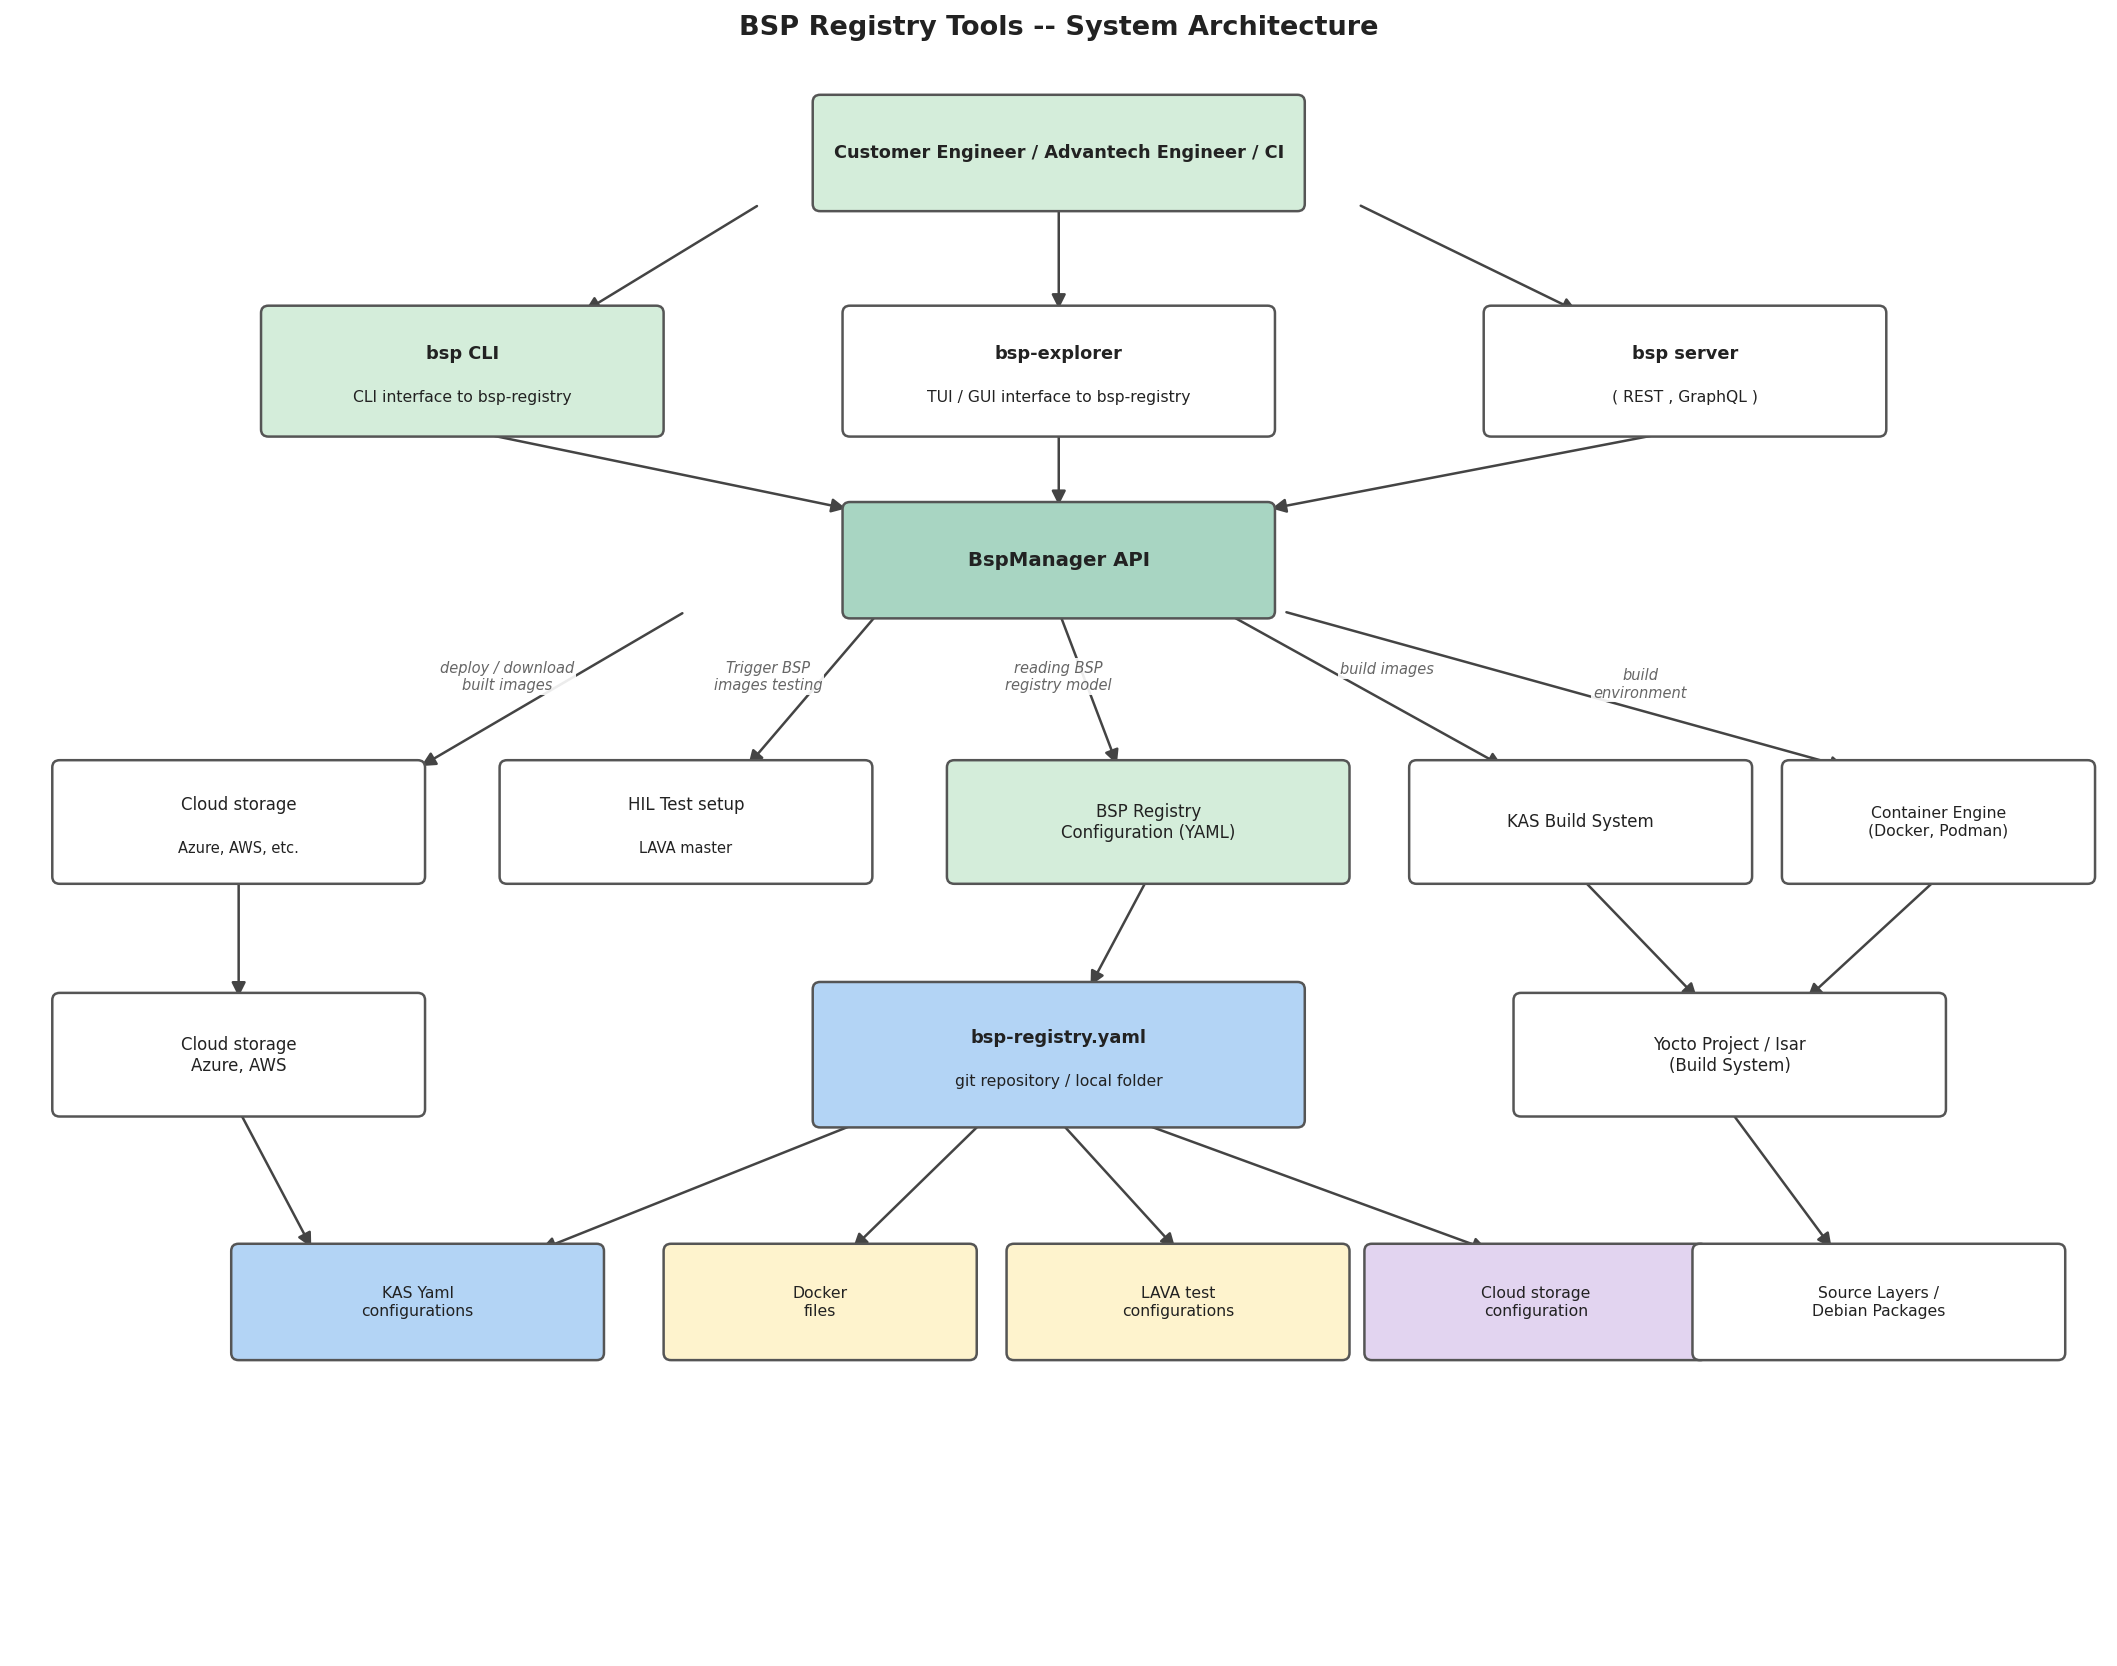
\includegraphics[width=\linewidth]{architecture.png}
  \caption{BSP Registry Tools --- System Architecture}
  \label{fig:arch}
\end{figure}

\subsection{Component Roles}

\begin{tabularx}{\linewidth}{L{50mm}X}
  \rowcolor{tableheadbg}
  \textbf{Component} & \textbf{Role} \\
  \toprule
  \rowcolor{roweven} bsp CLI
    & Primary user interface --- build, list, export, deploy, gather, registry CRUD \\
  \rowcolor{rowodd}  bsp-explorer
    & TUI / GUI interface (interactive terminal explorer) \\
  \rowcolor{roweven} bsp server
    & HTTP REST + GraphQL server for automation and dashboards \\
  \rowcolor{rowodd}  BspManager API
    & Core Python library coordinating all operations \\
  \rowcolor{roweven} BSP Registry YAML
    & Single source of truth: devices, releases, features, presets \\
  \rowcolor{rowodd}  KAS Build System
    & Orchestrates Yocto BitBake or Isar builds from YAML config files \\
  \rowcolor{roweven} Container Engine
    & Docker / Podman provides isolated, reproducible build environments \\
  \rowcolor{rowodd}  Cloud Storage
    & Azure Blob / AWS S3 for artifact upload (\texttt{deploy}) and download (\texttt{gather}) \\
  \rowcolor{roweven} HIL Test / LAVA
    & Hardware-in-the-loop test automation via LAVA \\
  \bottomrule
\end{tabularx}

% ─────────────────────────────────────────────────────────────────────────────
\section{Installation}

Python 3.8 or later is required. A virtual environment is strongly recommended.

\subsection{Core install}

\begin{lstlisting}[language=bash]
pip install bsp-registry-tools
\end{lstlisting}

\subsection{Optional extras}

\begin{tabularx}{\linewidth}{L{35mm}X}
  \rowcolor{tableheadbg}
  \textbf{Extra} & \textbf{Installs} \\
  \toprule
  \rowcolor{roweven} \texttt{[azure]}       & Azure Blob Storage upload / download \\
  \rowcolor{rowodd}  \texttt{[aws]}         & AWS S3 upload / download \\
  \rowcolor{roweven} \texttt{[server]}      & FastAPI + uvicorn + Strawberry GraphQL \\
  \rowcolor{rowodd}  \texttt{[completions]} & Shell tab completions (argcomplete) \\
  \rowcolor{roweven} \texttt{[dev]}         & pytest, coverage, ruff, \ldots \\
  \bottomrule
\end{tabularx}

\begin{lstlisting}[language=bash]
pip install "bsp-registry-tools[azure,completions]"
\end{lstlisting}

% ─────────────────────────────────────────────────────────────────────────────
\section{Supported Hardware}

\subsection{NXP i.MX Boards (Advantech Europe)}

\begin{tabularx}{\linewidth}{L{22mm}L{22mm}XL{22mm}}
  \rowcolor{tableheadbg}
  \textbf{Board} & \textbf{SoC} & \textbf{Yocto Releases} & \textbf{Status} \\
  \toprule
  \rowcolor{roweven} RSB-3720    & i.MX8M Plus & scarthgap, styhead, walnascar, whinlatter & Stable \\
  \rowcolor{rowodd}  RSB-3720 4G & i.MX8M Plus & walnascar, whinlatter                     & Stable \\
  \rowcolor{roweven} RSB-3720 6G & i.MX8M Plus & walnascar, whinlatter                     & Stable \\
  \rowcolor{rowodd}  ROM-2620    & i.MX8       & scarthgap, styhead, walnascar, whinlatter & Stable \\
  \rowcolor{roweven} ROM-2820    & i.MX93      & scarthgap, styhead, walnascar, whinlatter & Stable \\
  \rowcolor{rowodd}  ROM-5720    & i.MX8       & scarthgap, styhead, walnascar, whinlatter & Stable \\
  \rowcolor{roweven} ROM-5721    & i.MX8       & scarthgap, styhead, walnascar, whinlatter & Stable \\
  \rowcolor{rowodd}  ROM-5722    & i.MX8       & scarthgap, styhead, walnascar, whinlatter & Stable \\
  \rowcolor{roweven} AOM-5521    & i.MX95      & scarthgap, walnascar                      & Stable \\
  \bottomrule
\end{tabularx}

\subsection{MediaTek \& Qualcomm Boards}

\begin{tabularx}{\linewidth}{L{38mm}L{38mm}L{28mm}L{28mm}}
  \rowcolor{tableheadbg}
  \textbf{Board} & \textbf{SoC} & \textbf{Releases} & \textbf{Status} \\
  \toprule
  \rowcolor{roweven} RSB-3810         & MediaTek MT8395  & scarthgap & Development \\
  \rowcolor{rowodd}  Genio 1200 EVK   & MediaTek MT8395  & scarthgap & Development \\
  \rowcolor{roweven} AOM-2721         & Qualcomm QCS6490 & scarthgap & Development \\
  \rowcolor{rowodd}  QCS6490 RB3 Gen2 & Qualcomm QCS6490 & scarthgap & Development \\
  \bottomrule
\end{tabularx}

\subsection{Emulated Targets (QEMU)}

\begin{itemize}
  \item \texttt{qemuarm64} --- 64-bit ARM (AArch64)
  \item \texttt{qemuarm}   --- 32-bit ARM
  \item \texttt{qemux86}   --- x86 32-bit
  \item \texttt{qemux86-64} / \texttt{qemuamd64} --- x86-64
\end{itemize}

% ─────────────────────────────────────────────────────────────────────────────
\section{Supported Releases}

\subsection{Yocto Releases}

\begin{tabularx}{\linewidth}{L{28mm}L{24mm}L{12mm}X}
  \rowcolor{tableheadbg}
  \textbf{Slug} & \textbf{Yocto Version} & \textbf{LTS} & \textbf{Notes} \\
  \toprule
  \rowcolor{roweven} kirkstone  & 4.0 & LTS & poky, fsl-imx-xwayland \\
  \rowcolor{rowodd}  mickledore & 4.2 &     & poky, fsl-imx-xwayland \\
  \rowcolor{roweven} nanbield   & 4.3 &     & poky \\
  \rowcolor{rowodd}  scarthgap  & 5.0 & LTS & poky, fsl-imx-xwayland, mediatek, qualcomm, ros2 \\
  \rowcolor{roweven} styhead    & 5.1 &     & poky, fsl-imx-xwayland \\
  \rowcolor{rowodd}  walnascar  & 5.2 &     & poky, fsl-imx-xwayland \\
  \rowcolor{roweven} whinlatter & 5.3 &     & poky, fsl-imx-xwayland \\
  \rowcolor{rowodd}  wrynose    & 6.0 &     & poky (upcoming) \\
  \bottomrule
\end{tabularx}

\subsection{Isar (Debian-based) Releases}

\begin{tabularx}{\linewidth}{L{36mm}L{50mm}X}
  \rowcolor{tableheadbg}
  \textbf{Slug} & \textbf{Distribution} & \textbf{Base Image} \\
  \toprule
  \rowcolor{roweven} debian-trixie & Debian 13 (Trixie) & isar-debian-13 container \\
  \rowcolor{rowodd}  ubuntu-noble  & Ubuntu 24.04 LTS   & isar-debian-13 container \\
  \rowcolor{roweven} ubuntu-jammy  & Ubuntu 22.04 LTS   & isar-debian-13 container \\
  \bottomrule
\end{tabularx}

% ─────────────────────────────────────────────────────────────────────────────
\section{Registry Schema v2}

The registry uses a YAML file (default: \texttt{bsp-registry.yml}) with schema
version 2.0. The file decomposes into independent, reusable sections:

\begin{tabularx}{\linewidth}{L{36mm}X}
  \rowcolor{tableheadbg}
  \textbf{Section} & \textbf{Purpose} \\
  \toprule
  \rowcolor{roweven} \texttt{frameworks}   & Build-system definitions (Yocto, Isar) \\
  \rowcolor{rowodd}  \texttt{distro}       & Distribution definitions (Poky, fsl-imx-xwayland, \ldots) \\
  \rowcolor{roweven} \texttt{vendors}      & Cross-release board-vendor KAS fragments \\
  \rowcolor{rowodd}  \texttt{devices}      & Hardware board definitions (slug, vendor, SoC, KAS includes) \\
  \rowcolor{roweven} \texttt{releases}     & Yocto / Isar release definitions with vendor overrides \\
  \rowcolor{rowodd}  \texttt{features}     & Optional add-ons (OTA, secure-boot, ROS 2, hailo, \ldots) \\
  \rowcolor{roweven} \texttt{bsp}          & Named presets = device + release(s) + features \\
  \rowcolor{rowodd}  \texttt{environments} & Container + variable bundles per build class \\
  \rowcolor{roweven} \texttt{containers}   & Docker image definitions \\
  \rowcolor{rowodd}  \texttt{deploy}       & Cloud artifact upload configuration (Azure / AWS) \\
  \rowcolor{roweven} \texttt{include}      & Split large registries across multiple files \\
  \bottomrule
\end{tabularx}

\subsection{Device Definition Example}

\begin{lstlisting}[language={}]
registry:
  devices:
    - slug: rsb3720
      description: "Advantech RSB-3720 (i.MX8M Plus, 6GB)"
      vendor: advantech-europe
      soc_vendor: nxp
      architecture: arm64
      includes:
        - vendors/advantech-europe/nxp/machine/imx8/rsb3720.yml
\end{lstlisting}

\subsection{Named Preset Example}

\begin{lstlisting}[language={}]
registry:
  bsp:
    - name: modular-bsp-rsb3720
      description: "Advantech RSB-3720 (i.MX8)"
      device: rsb3720
      releases: [scarthgap, styhead, walnascar, whinlatter]
      features: [systemd, security, virtualization, ipv6, usrmerge]
      build:
        path: build/modular-bsp-rsb3720
\end{lstlisting}

\subsection{Vendor Override Example}

Vendor overrides allow a single release slug (e.g.\ \texttt{scarthgap}) to apply
different KAS fragments and distro settings per hardware vendor / SoC combination,
with optional kernel sub-release pinning:

\begin{lstlisting}[language={}]
releases:
  - slug: scarthgap
    distro: poky
    includes:
      - compilers/clang/clang.yml
      - yocto/releases/scarthgap.yml
    vendor_overrides:
      - vendor: advantech-europe
        soc_vendors:
          - vendor: nxp
            distro: fsl-imx-xwayland
            includes:
              - vendors/advantech-europe/nxp/modular-bsp-nxp.yml
            releases:
              - slug: imx-6.6.52-2.2.2
                includes:
                  - vendors/advantech-europe/nxp/imx-6.6.52-2.2.2-scarthgap.yml
\end{lstlisting}

% ─────────────────────────────────────────────────────────────────────────────
\section{Feature System}

Features are optional, composable add-ons that can be mixed into any BSP preset.
They support \texttt{vendor\_overrides} and \texttt{release\_overrides} so the correct
KAS fragments are injected automatically based on the target hardware and Yocto release.

\begin{tabularx}{\linewidth}{L{34mm}X}
  \rowcolor{tableheadbg}
  \textbf{Slug} & \textbf{Description} \\
  \toprule
  \rowcolor{roweven} \texttt{systemd}      & Enable systemd as the init system \\
  \rowcolor{rowodd}  \texttt{yocto-ssh}    & Include SSH server in the image \\
  \rowcolor{roweven} \texttt{debug-tweaks} & Enable debug build tweaks (empty root password, \ldots) \\
  \rowcolor{rowodd}  \texttt{root-login}   & Enable root login \\
  \rowcolor{roweven} \texttt{security}     & Security hardening meta-layer \\
  \rowcolor{rowodd}  \texttt{secure-boot}  & NXP HAB / AHAB cryptographic image signing \\
  \rowcolor{roweven} \texttt{virtualization} & KVM / container virtualisation support \\
  \rowcolor{rowodd}  \texttt{wayland}      & Wayland display server support \\
  \rowcolor{roweven} \texttt{x11}          & X11 display server support \\
  \rowcolor{rowodd}  \texttt{ipv6}         & IPv6 networking \\
  \rowcolor{roweven} \texttt{udev}         & udev device manager \\
  \rowcolor{rowodd}  \texttt{usrmerge}     & /usr merge (FHS compliance) \\
  \rowcolor{roweven} \texttt{rauc}         & RAUC Over-the-Air update framework \\
  \rowcolor{rowodd}  \texttt{swupdate}     & SWUpdate OTA framework \\
  \rowcolor{roweven} \texttt{ostree}       & OSTree atomic filesystem upgrades \\
  \rowcolor{rowodd}  \texttt{hailo}        & Hailo-8 AI accelerator support \\
  \rowcolor{roweven} \texttt{ros2}         & ROS 2 via ros2-humble-scarthgap release \\
  \bottomrule
\end{tabularx}

% ─────────────────────────────────────────────────────────────────────────────
\section{OTA Update Support}

Three OTA technologies are supported as first-class composable features.
All major Advantech Europe NXP boards support all three methods.

\begin{tabularx}{\linewidth}{L{22mm}L{20mm}XL{35mm}}
  \rowcolor{tableheadbg}
  \textbf{Technology} & \textbf{Slug} & \textbf{Supported Boards} & \textbf{Releases} \\
  \toprule
  \rowcolor{roweven} RAUC
    & \texttt{rauc}
    & RSB-3720, ROM-2620, ROM-2820, ROM-5720/21/22
    & scarthgap -- whinlatter \\
  \rowcolor{rowodd}  SWUpdate
    & \texttt{swupdate}
    & RSB-3720, ROM-2620, ROM-2820, ROM-5720/21/22
    & scarthgap -- whinlatter \\
  \rowcolor{roweven} OSTree
    & \texttt{ostree}
    & RSB-3720, ROM-2620, ROM-2820, ROM-5720/21/22
    & scarthgap -- whinlatter \\
  \bottomrule
\end{tabularx}

\begin{lstlisting}[language=bash]
# Build RSB-3720 with RAUC OTA (Walnascar release)
bsp build modular-bsp-rauc-rsb3720 --release walnascar

# Build RSB-3720 with SWUpdate
bsp build modular-bsp-swupdate-rsb3720 --release scarthgap

# Build RSB-3720 with OSTree
bsp build modular-bsp-ostree-rsb3720 --release walnascar
\end{lstlisting}

% ─────────────────────────────────────────────────────────────────────────────
\section{Secure Boot}

NXP-based Advantech boards support cryptographic boot-image signing via HAB
(i.MX8 family) and AHAB (i.MX9 / i.MX95 family). The \texttt{secure-boot}
feature uses the \texttt{ubuntu-22.04-csb} container which automatically mounts
the NXP CST signing tool and keys from the host into the container.

\begin{tabularx}{\linewidth}{L{22mm}L{56mm}X}
  \rowcolor{tableheadbg}
  \textbf{SoC Family} & \textbf{Technology} & \textbf{Boards} \\
  \toprule
  \rowcolor{roweven} i.MX8  & HAB (High Assurance Boot)            & RSB-3720, ROM-2620, ROM-5720, ROM-5721, ROM-5722 \\
  \rowcolor{rowodd}  i.MX93 & AHAB (Advanced High Assurance Boot)  & ROM-2820 \\
  \rowcolor{roweven} i.MX95 & AHAB                                  & AOM-5521 \\
  \bottomrule
\end{tabularx}

\begin{lstlisting}[language=bash]
# Export signing key environment variables
export CST_TOOL_PATH=/opt/nxp/cst/
export KEYS_PATH=/path/to/srk-keys/

# Build ROM-5721 2G with Secure Boot (uses ubuntu-22.04-csb container)
bsp build modular-bsp-rom5721-2g-db5901-secureboot --release walnascar
\end{lstlisting}

% ─────────────────────────────────────────────────────────────────────────────
\section{Containers \& Environments}

Container definitions bundle a Dockerfile, a Docker image name, build args, and
optional volume mounts. Named environments combine a container with build-system
environment variables.

\begin{tabularx}{\linewidth}{L{38mm}L{26mm}L{18mm}X}
  \rowcolor{tableheadbg}
  \textbf{Container} & \textbf{Base OS} & \textbf{KAS} & \textbf{Use Case} \\
  \toprule
  \rowcolor{roweven} ubuntu-20.04     & Ubuntu 20.04 & 4.7 & Kirkstone / Mickledore legacy builds \\
  \rowcolor{rowodd}  ubuntu-22.04     & Ubuntu 22.04 & 5.2 & Default Yocto builds \\
  \rowcolor{roweven} ubuntu-22.04-csb & Ubuntu 22.04 & 5.2 & Secure Boot builds (key mounts) \\
  \rowcolor{rowodd}  ubuntu-24.04     & Ubuntu 24.04 & 5.2 & Latest Yocto builds \\
  \rowcolor{roweven} debian-12        & Debian 12    & 5.2 & Hardened / alternative builds \\
  \rowcolor{rowodd}  debian-13        & Debian 13    & 5.2 & Debian-based Yocto builds \\
  \rowcolor{roweven} isar-debian-13   & Debian 13    & 5.2 & Isar privileged builds \\
  \bottomrule
\end{tabularx}

% ─────────────────────────────────────────────────────────────────────────────
\section{CLI Reference}

\begin{tabularx}{\linewidth}{L{78mm}X}
  \rowcolor{tableheadbg}
  \textbf{Command} & \textbf{Description} \\
  \toprule
  \rowcolor{roweven} \texttt{bsp list}                              & List all named BSP presets \\
  \rowcolor{rowodd}  \texttt{bsp list devices}                     & List all device slugs \\
  \rowcolor{roweven} \texttt{bsp list releases}                    & List all release slugs \\
  \rowcolor{rowodd}  \texttt{bsp list features}                    & List all feature slugs \\
  \rowcolor{roweven} \texttt{bsp containers}                       & List container definitions \\
  \rowcolor{rowodd}  \texttt{bsp build <preset>}                   & Build a named preset \\
  \rowcolor{roweven} \texttt{bsp build <preset> --release <r>}     & Build with a specific release \\
  \rowcolor{rowodd}  \texttt{bsp build <preset> --checkout}        & Validate config (no actual build) \\
  \rowcolor{roweven} \texttt{bsp build <preset> --deploy}          & Build and deploy to cloud storage \\
  \rowcolor{rowodd}  \texttt{bsp build <preset> --clean}           & Clean build dir before building \\
  \rowcolor{roweven} \texttt{bsp shell <preset>}                   & Open shell in build container \\
  \rowcolor{rowodd}  \texttt{bsp export <preset>}                  & Export resolved KAS config \\
  \rowcolor{roweven} \texttt{bsp deploy <preset>}                  & Upload artifacts to cloud storage \\
  \rowcolor{rowodd}  \texttt{bsp gather <preset>}                  & Download artifacts from cloud \\
  \rowcolor{roweven} \texttt{bsp registry init}                    & Scaffold a new registry YAML file \\
  \rowcolor{rowodd}  \texttt{bsp registry validate}                & Validate registry schema \\
  \rowcolor{roweven} \texttt{bsp registry diff <f1> <f2>}          & Diff between two registry files \\
  \rowcolor{rowodd}  \texttt{bsp registry add device ...}          & Add a new device entry \\
  \rowcolor{roweven} \texttt{bsp registry add release ...}         & Add a new release entry \\
  \rowcolor{rowodd}  \texttt{bsp remotes add <name> <url>}         & Save a named remote registry URL \\
  \rowcolor{roweven} \texttt{bsp remotes show}                     & List all saved remotes \\
  \rowcolor{rowodd}  \texttt{bsp server}                           & Start REST + GraphQL HTTP server \\
  \rowcolor{roweven} \texttt{bsp completions bash|zsh|fish}        & Print shell completion script \\
  \bottomrule
\end{tabularx}

\subsection{Global CLI Flags}

\begin{tabularx}{\linewidth}{L{46mm}X}
  \rowcolor{tableheadbg}
  \textbf{Flag} & \textbf{Description} \\
  \toprule
  \rowcolor{roweven} \texttt{--registry <path>} & Use an explicit local registry file \\
  \rowcolor{rowodd}  \texttt{--local}           & Use \texttt{./bsp-registry.yml}, no network \\
  \rowcolor{roweven} \texttt{--remote <url>}    & Remote registry URL or saved remote name \\
  \rowcolor{rowodd}  \texttt{--branch <b>}      & Branch to checkout when using \texttt{--remote} \\
  \rowcolor{roweven} \texttt{--no-update}       & Skip git-pull of the remote registry \\
  \bottomrule
\end{tabularx}

\subsection{Quick Start}

\begin{lstlisting}[language=bash]
# First run: clones the Advantech registry automatically
bsp list

# Build Advantech RSB-3720 with the default release
bsp build modular-bsp-rsb3720

# Build with a specific Yocto release
bsp build modular-bsp-rsb3720 --release walnascar

# Validate config quickly (no full build)
bsp build modular-bsp-rsb3720 --checkout

# Use the Advantech development branch explicitly
bsp --remote https://github.com/Advantech-EECC/bsp-registry.git@development list
\end{lstlisting}

% ─────────────────────────────────────────────────────────────────────────────
\section{Python API}

All CLI operations are backed by a public Python API.  The key entry point is
\texttt{BspManager}, which coordinates registry loading, preset resolution, builds,
deployment, and artifact gathering.

\begin{lstlisting}[language=python]
from bsp import BspManager, RegistryFetcher, V2Resolver

# 1. Fetch / update the remote registry
fetcher = RegistryFetcher()
registry_path = fetcher.fetch_registry(
    repo_url="https://github.com/Advantech-EECC/bsp-registry.git",
    branch="development",
    update=True,
)

# 2. Load registry and inspect contents
manager = BspManager(str(registry_path))
manager.initialize()
for dev in manager.model.registry.devices:
    print(dev.slug, dev.description)

# 3. Resolve a preset into a full build configuration
resolver = V2Resolver(manager.model)
config = resolver.resolve(
    device_slug="rsb3720",
    release_slug="walnascar",
    feature_slugs=["systemd", "security", "rauc"],
)
for f in config.kas_files:
    print(f)
\end{lstlisting}

\subsection{Multi-Registry Mode}

\begin{lstlisting}[language=python]
from bsp import BspManager

manager = BspManager(
    config_paths=[
        ("advantech",    "/path/to/advantech-registry.yaml"),
        ("my-additions", "/path/to/my-registry.yaml"),
    ]
)
manager.initialize()
# Disambiguate with registry:preset syntax
config = manager.resolve("advantech:modular-bsp-rsb3720")
\end{lstlisting}

% ─────────────────────────────────────────────────────────────────────────────
\section{HTTP Server (REST + GraphQL)}

\begin{lstlisting}[language=bash]
pip install "bsp-registry-tools[server]"
bsp server --port 8080
\end{lstlisting}

\subsection{REST API Endpoints}

\begin{tabularx}{\linewidth}{L{14mm}L{64mm}X}
  \rowcolor{tableheadbg}
  \textbf{Method} & \textbf{Path} & \textbf{Description} \\
  \toprule
  \rowcolor{roweven} GET  & \texttt{/api/v1/devices}          & List all devices \\
  \rowcolor{rowodd}  GET  & \texttt{/api/v1/releases}         & List all releases \\
  \rowcolor{roweven} GET  & \texttt{/api/v1/features}         & List all features \\
  \rowcolor{rowodd}  GET  & \texttt{/api/v1/bsp}              & List all named presets \\
  \rowcolor{roweven} POST & \texttt{/api/v1/bsp/\{name\}/build} & Trigger a build \\
  \rowcolor{rowodd}  POST & \texttt{/graphql}                 & GraphQL endpoint \\
  \bottomrule
\end{tabularx}

\begin{lstlisting}[language=bash]
# GraphQL query example
curl -X POST http://localhost:8080/graphql \
  -H 'Content-Type: application/json' \
  -d '{"query": "{ releases { slug description yoctoVersion } }"}'
\end{lstlisting}

% ─────────────────────────────────────────────────────────────────────────────
\section{CI/CD Integration}

\begin{lstlisting}[language={}]
# .github/workflows/build.yml
jobs:
  build:
    runs-on: ubuntu-latest
    steps:
      - uses: actions/checkout@v4

      - name: Install bsp-registry-tools
        run: pip install "bsp-registry-tools[azure]"

      - name: Validate registry
        run: bsp --local registry validate

      - name: Fast checkout gate (no full build)
        run: bsp --no-update build modular-bsp-rsb3720 --checkout

      - name: Build and deploy artifacts
        env:
          AZURE_STORAGE_ACCOUNT_URL: ${{ secrets.AZURE_STORAGE_ACCOUNT_URL }}
        run: bsp --no-update build modular-bsp-rsb3720 --release walnascar --deploy
\end{lstlisting}

% ─────────────────────────────────────────────────────────────────────────────
\section{Extending BSPs with Custom Yocto Layers}

A BSP registry KAS configuration can be included in your own project,
allowing you to add custom Yocto layers on top of an existing BSP without
modifying the registry itself.

\begin{lstlisting}[language={}]
# my-custom-kas.yaml
header:
  version: 19
  includes:
    - repo: bsp-registry
      file: modular-bsp-rsb3720-walnascar.yaml   # from `bsp export`

repos:
  bsp-registry:
    url: "https://github.com/Advantech-EECC/bsp-registry"
    branch: "development"
    layers: { .: "disabled" }

  meta-custom:
    layers:
      meta-custom:    # your custom Yocto meta-layer
\end{lstlisting}

\begin{lstlisting}[language=bash]
# meta-custom/meta-custom/recipes-core/imx-image-%.bbappend
CORE_IMAGE_EXTRA_INSTALL += "mpv"
LICENSE_FLAGS_ACCEPTED += "commercial"

# Build with your extension
kas build my-custom-kas.yaml
\end{lstlisting}

% ─────────────────────────────────────────────────────────────────────────────
\section{Summary}

\begin{tabularx}{\linewidth}{L{50mm}X}
  \rowcolor{tableheadbg}
  \textbf{Feature} & \textbf{Benefit} \\
  \toprule
  \rowcolor{roweven} YAML registry v2         & Single source of truth for 30+ boards $\times$ 8+ releases \\
  \rowcolor{rowodd}  Auto remote fetch        & Zero-config first run; teams share the Advantech registry \\
  \rowcolor{roweven} Two build systems        & Yocto/BitBake AND Isar/Debian in one registry \\
  \rowcolor{rowodd}  KAS integration          & Reproducible builds for every device $\times$ release combo \\
  \rowcolor{roweven} Named environments       & Correct container per build class (secure-boot, Isar, \ldots) \\
  \rowcolor{rowodd}  Feature system           & Composable add-ons: OTA, secure-boot, ROS 2, Hailo \\
  \rowcolor{roweven} OTA support              & RAUC, SWUpdate, OSTree --- all first-class features \\
  \rowcolor{rowodd}  Secure Boot              & NXP HAB / AHAB signing built into the registry \\
  \rowcolor{roweven} Cloud deploy / gather    & Full artifact lifecycle: build $\to$ upload $\to$ download \\
  \rowcolor{rowodd}  HTTP server              & REST + GraphQL for dashboards and automation \\
  \rowcolor{roweven} Tab completions          & Fast CLI use with context-aware completions \\
  \rowcolor{rowodd}  Python API               & Integrate into custom tools and CI scripts \\
  \bottomrule
\end{tabularx}

\vspace{8mm}
\begin{center}
  \small\itshape
  Registry: \url{https://github.com/Advantech-EECC/bsp-registry} (development branch)
\end{center}

\end{document}
